% **************************PAPER COMMENTS***********************

% Ended up keeping non-PR works, so this was commented out. Would have been used as a limitation:
% Before reading and conducting IRR measures on the full papers, the authors decided on an additional exclusion criterion: papers that were not published to peer reviewed conferences or journals would not be included in our final corpus. This meant that all works emanating from sources that were not peer reviewed, workshops, and books would be excluded from the corpus. A large impetus for this decision was the plethora of relevant works already peer reviewed, published, and available. While novel fields and approaches may necessitate the inclusion of works that have not yet gone through the peer review process due to the subject's novelty or a dearth of peer reviewed publications, our literature search informed us this was not the case for the domain of multimodal learning and training environments. The decision not to include books was made out of pragmatism: given the time cost of reading complete books, the authors elected not to include them in the final corpus so as to ensure timely publication and relative novelty of the review. 

% Old modality definition
% A \textit{modality} is defined by a single datastream from one data collection source (camera lens, microphone, sensor, etc.), or the combination of multiple data collection sources (inertial measurement unit (IMU) sensor, for example), where that datastream is used for analysis. 

% I'm not sure if the below RQs were options for us or if they were RQs from other works. Eduardo, do you have any idea?
%   RQ1: What is the existing evidence on the use of MMLA systems to support educational outcomes in real-world settings? 
%   RQ2: To what extent ethical considerations are highlighted and addressed in MMLA research? 
% Multimodal data capabilities for learning: What can multimodal data tell us about learning?
%   RQ1: What is the current status of MMD for learning research, seen through the lens of areas of implementation (e.g., learning scenario, learning environments), technologies used and methodologies (e.g., types of data and data analysis techniques)? 
%   RQ2: What insights the MMD has given us about learning (i.e., MMD capabilities for learning)?
% Trends of Multimodal Learning Analytics: A Systematic Literature Review    
%   RQ1: What is the current state of the art of Multimodal Learning Analytics? 
%   RQ2: What are the existing Multimodal Learning Analytics methods are being used in Education sectors? 
%   RQ3: What are the challenges of Multimodal Learning Analytics in leveraging various learning practices?

% Not interested in VR, so this came out
% Multimodal teaching, learning and training in virtual reality: a review and case study
%   Focus on VR, specifically
%   11 industry case studies
%   References findings from other SLRs in intro
%   Defines multimodality as: “Multimodality refers to ‘multiple’ modes of representation, with combined elements of print, visual images and design.” No citation
%   Focus on practice, feedback, evaluation, knowledge transmission

% These subsections of "Findings" were taken out due to us no longer focusing on them
% \subsection{Feedback Systems}
% \subsection{XAI}
% \subsubsection{Privacy}
% \subsubsection{Security}
% \subsubsection{Robustness}

% Commented out after deciding to keep papers not peer reviewed
% The major limitations of this work involve the use of Google Scholar to conduct the literature search, the use of a citation graph for programmatic corpus reduction, and our choice to not include works in the corpus that had not been peer reviewed at the time of the literature search. All three are discussed in the following paragraphs.

% Commented out after deciding to keep papers not peer reviewed
% \subsubsection{Works not (yet) peer reviewed.} 
% While it has been historically accepted to include only peer reviewed publications in literature reviews to ensure corpus quality, it is becoming commonplace for (usually private) institutions to publish major findings to open access databases without going through the formal peer review process. In many cases, these publications are seminal works that represent paradigm shifts in entire fields of research. Google's language model BERT\footnote{Bidirectional Encoder Representations from Transformers} \cite{devlin2018bert}, for example, was a seminal work in 2018 that has since been cited over 58,000 times as of the writing of this paper. However, the paper's authors published the findings to arXiv\footnote{\href{https://arxiv.org/}{https://arxiv.org/}}, which is an open access research database whose works do not undergo peer review. Similarly, another language model, ChatGPT\footnote{\href{https://openai.com/blog/chatgpt/}{https://openai.com/blog/chatgpt/}} was published via blog post but has already enjoyed a considerable amount of ubiquity even outside of academia. Despite their influence on the field, both of these innovations would be ineligible for inclusion based on our criterion even if they were relevant to this review.

% We deviated from the below diagram, but we can update it if we want to reinclude it
% \begin{figure}
%     \centering
%     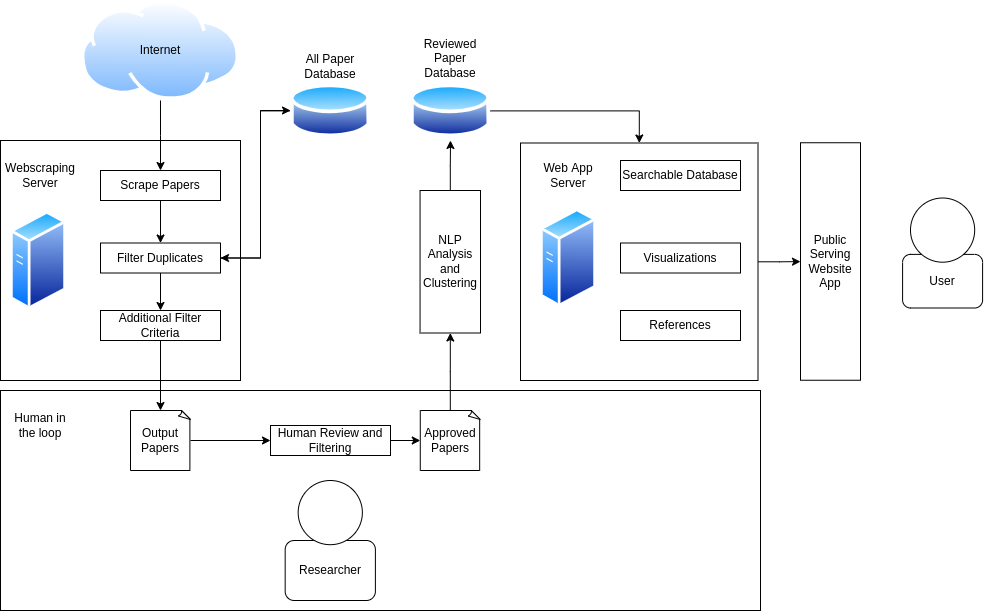
\includegraphics[width=\textwidth]{img/Architecture.drawio.png}
%     \caption{Paper Processing Architecture}
%     \label{fig:architecture}
% \end{figure}

% I wasn't sure where this image was supposed to fit it, but we can discuss if we have a place for it
% \begin{figure}
%     \centering
%     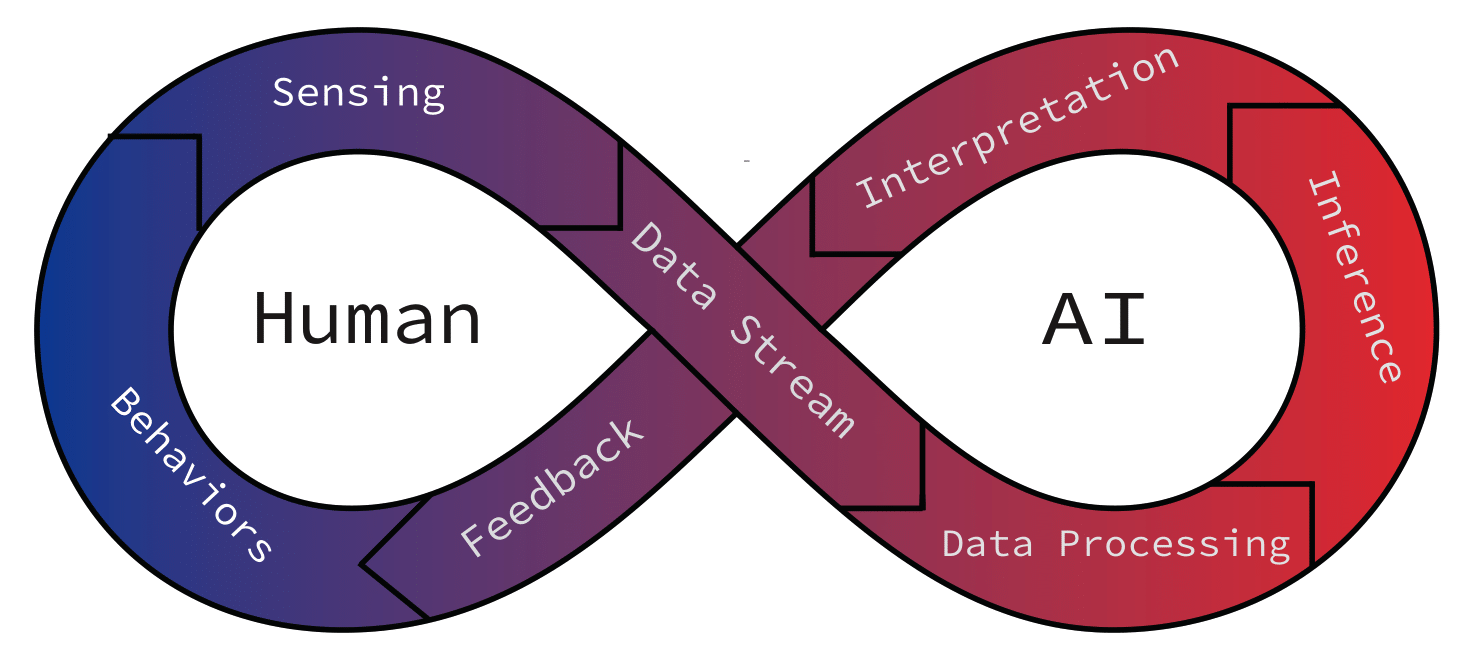
\includegraphics[width=\textwidth]{img/infinity_diagram.png}
%     \caption{Infinity diagram}
%     \label{fig:infinity}
% \end{figure}


% **************************TEMPLATE COMMENTS***********************

%%
%% This is file `sample-manuscript.tex',
%% generated with the docstrip utility.
%%
%% The original source files were:
%%
%% samples.dtx  (with options: `manuscript')
%% 
%% IMPORTANT NOTICE:
%% 
%% For the copyright see the source file.
%% 
%% Any modified versions of this file must be renamed
%% with new filenames distinct from sample-manuscript.tex.
%% 
%% For distribution of the original source see the terms
%% for copying and modification in the file samples.dtx.
%% 
%% This generated file may be distributed as long as the
%% original source files, as listed above, are part of the
%% same distribution. (The sources need not necessarily be
%% in the same archive or directory.)
%%
%%
%% Commands for TeXCount
%TC:macro \cite [option:text,text]
%TC:macro \citep [option:text,text]
%TC:macro \citet [option:text,text]
%TC:envir table 0 1
%TC:envir table* 0 1
%TC:envir tabular [ignore] word
%TC:envir displaymath 0 word
%TC:envir math 0 word
%TC:envir comment 0 0
%%
%%
%% The first command in your LaTeX source must be the \documentclass
%% command.
%%
%% For submission and review of your manuscript please change the
%% command to \documentclass[manuscript, screen, review]{acmart}.
%%
%% When submitting camera ready or to TAPS, please change the command
%% to \documentclass[sigconf]{acmart} or whichever template is required
%% for your publication.
%%
%%

% Author template comments:

% \author{Ben Trovato}
% \authornote{Both authors contributed equally to this research.}
% \email{trovato@corporation.com}
% \orcid{1234-5678-9012}
% \author{G.K.M. Tobin}
% \authornotemark[1]
% \email{webmaster@marysville-ohio.com}
% \affiliation{%
%   \institution{Institute for Clarity in Documentation}
%   \streetaddress{P.O. Box 1212}
%   \city{Dublin}
%   \state{Ohio}
%   \country{USA}
%   \postcode{43017-6221}
% }

% \author{Lars Th{\o}rv{\"a}ld}
% \affiliation{%
%   \institution{The Th{\o}rv{\"a}ld Group}
%   \streetaddress{1 Th{\o}rv{\"a}ld Circle}
%   \city{Hekla}
%   \country{Iceland}}
% \email{larst@affiliation.org}

% \author{Valerie B\'eranger}
% \affiliation{%
%   \institution{Inria Paris-Rocquencourt}
%   \city{Rocquencourt}
%   \country{France}
% }

% \author{Aparna Patel}
% \affiliation{%
%  \institution{Rajiv Gandhi University}
%  \streetaddress{Rono-Hills}
%  \city{Doimukh}
%  \state{Arunachal Pradesh}
%  \country{India}}

% \author{Huifen Chan}
% \affiliation{%
%   \institution{Tsinghua University}
%   \streetaddress{30 Shuangqing Rd}
%   \city{Haidian Qu}
%   \state{Beijing Shi}
%   \country{China}}

% \author{Charles Palmer}
% \affiliation{%
%   \institution{Palmer Research Laboratories}
%   \streetaddress{8600 Datapoint Drive}
%   \city{San Antonio}
%   \state{Texas}
%   \country{USA}
%   \postcode{78229}}
% \email{cpalmer@prl.com}

% \author{John Smith}
% \affiliation{%
%   \institution{The Th{\o}rv{\"a}ld Group}
%   \streetaddress{1 Th{\o}rv{\"a}ld Circle}
%   \city{Hekla}
%   \country{Iceland}}
% \email{jsmith@affiliation.org}

% \author{Julius P. Kumquat}
% \affiliation{%
%   \institution{The Kumquat Consortium}
%   \city{New York}
%   \country{USA}}
% \email{jpkumquat@consortium.net}

%%
%% By default, the full list of authors will be used in the page
%% headers. Often, this list is too long, and will overlap
%% other information printed in the page headers. This command allows
%% the author to define a more concise list
%% of authors' names for this purpose.

% Citation management

%%
%% For managing citations, it is recommended to use bibliography
%% files in BibTeX format.
%%
%% You can then either use BibTeX with the ACM-Reference-Format style,
%% or BibLaTeX with the acmnumeric or acmauthoryear sytles, that include
%% support for advanced citation of software artefact from the
%% biblatex-software package, also separately available on CTAN.
%%
%% Look at the sample-*-biblatex.tex files for templates showcasing
%% the biblatex styles.
%%

%%
%% The majority of ACM publications use numbered citations and
%% references.  The command \citestyle{authoryear} switches to the
%% "author year" style.
%%
%% If you are preparing content for an event
%% sponsored by ACM SIGGRAPH, you must use the "author year" style of
%% citations and references.
%% Uncommenting
%% the next command will enable that style.
%%\citestyle{acmauthoryear}


% Main template body commented out

% \begin{abstract}
%   A clear and well-documented \LaTeX\ document is presented as an
%   article formatted for publication by ACM in a conference proceedings
%   or journal publication. Based on the ``acmart'' document class, this
%   article presents and explains many of the common variations, as well
%   as many of the formatting elements an author may use in the
%   preparation of the documentation of their work.
% \end{abstract}

% \section{Introduction}
% ACM's consolidated article template, introduced in 2017, provides a
% consistent \LaTeX\ style for use across ACM publications, and
% incorporates accessibility and metadata-extraction functionality
% necessary for future Digital Library endeavors. Numerous ACM and
% SIG-specific \LaTeX\ templates have been examined, and their unique
% features incorporated into this single new template.

% If you are new to publishing with ACM, this document is a valuable
% guide to the process of preparing your work for publication. If you
% have published with ACM before, this document provides insight and
% instruction into more recent changes to the article template.

% The ``\verb|acmart|'' document class can be used to prepare articles
% for any ACM publication --- conference or journal, and for any stage
% of publication, from review to final ``camera-ready'' copy, to the
% author's own version, with {\itshape very} few changes to the source.

% \section{Template Overview}
% As noted in the introduction, the ``\verb|acmart|'' document class can
% be used to prepare many different kinds of documentation --- a
% double-blind initial submission of a full-length technical paper, a
% two-page SIGGRAPH Emerging Technologies abstract, a ``camera-ready''
% journal article, a SIGCHI Extended Abstract, and more --- all by
% selecting the appropriate {\itshape template style} and {\itshape
%   template parameters}.

% This document will explain the major features of the document
% class. For further information, the {\itshape \LaTeX\ User's Guide} is
% available from
% \url{https://www.acm.org/publications/proceedings-template}.

% \subsection{Template Styles}

% The primary parameter given to the ``\verb|acmart|'' document class is
% the {\itshape template style} which corresponds to the kind of publication
% or SIG publishing the work. This parameter is enclosed in square
% brackets and is a part of the {\verb|documentclass|} command:
% \begin{verbatim}
%   \documentclass[STYLE]{acmart}
% \end{verbatim}

% Journals use one of three template styles. All but three ACM journals
% use the {\verb|acmsmall|} template style:
% \begin{itemize}
% \item {\texttt{acmsmall}}: The default journal template style.
% \item {\texttt{acmlarge}}: Used by JOCCH and TAP.
% \item {\texttt{acmtog}}: Used by TOG.
% \end{itemize}

% The majority of conference proceedings documentation will use the {\verb|acmconf|} template style.
% \begin{itemize}
% \item {\texttt{acmconf}}: The default proceedings template style.
% \item{\texttt{sigchi}}: Used for SIGCHI conference articles.
% \item{\texttt{sigplan}}: Used for SIGPLAN conference articles.
% \end{itemize}

% \subsection{Template Parameters}

% In addition to specifying the {\itshape template style} to be used in
% formatting your work, there are a number of {\itshape template parameters}
% which modify some part of the applied template style. A complete list
% of these parameters can be found in the {\itshape \LaTeX\ User's Guide.}

% Frequently-used parameters, or combinations of parameters, include:
% \begin{itemize}
% \item {\texttt{anonymous,review}}: Suitable for a ``double-blind''
%   conference submission. Anonymizes the work and includes line
%   numbers. Use with the \texttt{\acmSubmissionID} command to print the
%   submission's unique ID on each page of the work.
% \item{\texttt{authorversion}}: Produces a version of the work suitable
%   for posting by the author.
% \item{\texttt{screen}}: Produces colored hyperlinks.
% \end{itemize}

% This document uses the following string as the first command in the
% source file:
% \begin{verbatim}
% \documentclass[manuscript,screen,review]{acmart}
% \end{verbatim}

% \section{Modifications}

% Modifying the template --- including but not limited to: adjusting
% margins, typeface sizes, line spacing, paragraph and list definitions,
% and the use of the \verb|\vspace| command to manually adjust the
% vertical spacing between elements of your work --- is not allowed.

% {\bfseries Your document will be returned to you for revision if
%   modifications are discovered.}

% \section{Typefaces}

% The ``\verb|acmart|'' document class requires the use of the
% ``Libertine'' typeface family. Your \TeX\ installation should include
% this set of packages. Please do not substitute other typefaces. The
% ``\verb|lmodern|'' and ``\verb|ltimes|'' packages should not be used,
% as they will override the built-in typeface families.

% \section{Title Information}

% The title of your work should use capital letters appropriately -
% \url{https://capitalizemytitle.com/} has useful rules for
% capitalization. Use the {\verb|title|} command to define the title of
% your work. If your work has a subtitle, define it with the
% {\verb|subtitle|} command.  Do not insert line breaks in your title.

% If your title is lengthy, you must define a short version to be used
% in the page headers, to prevent overlapping text. The \verb|title|
% command has a ``short title'' parameter:
% \begin{verbatim}
%   \title[short title]{full title}
% \end{verbatim}

% \section{Authors and Affiliations}

% Each author must be defined separately for accurate metadata
% identification.  As an exception, multiple authors may share one
% affiliation. Authors' names should not be abbreviated; use full first
% names wherever possible. Include authors' e-mail addresses whenever
% possible.

% Grouping authors' names or e-mail addresses, or providing an ``e-mail
% alias,'' as shown below, is not acceptable:
% \begin{verbatim}
%   \author{Brooke Aster, David Mehldau}
%   \email{dave,judy,steve@university.edu}
%   \email{firstname.lastname@phillips.org}
% \end{verbatim}

% The \verb|authornote| and \verb|authornotemark| commands allow a note
% to apply to multiple authors --- for example, if the first two authors
% of an article contributed equally to the work.

% If your author list is lengthy, you must define a shortened version of
% the list of authors to be used in the page headers, to prevent
% overlapping text. The following command should be placed just after
% the last \verb|\author{}| definition:
% \begin{verbatim}
%   \renewcommand{\shortauthors}{McCartney, et al.}
% \end{verbatim}
% Omitting this command will force the use of a concatenated list of all
% of the authors' names, which may result in overlapping text in the
% page headers.

% The article template's documentation, available at
% \url{https://www.acm.org/publications/proceedings-template}, has a
% complete explanation of these commands and tips for their effective
% use.

% Note that authors' addresses are mandatory for journal articles.

% \section{Rights Information}

% Authors of any work published by ACM will need to complete a rights
% form. Depending on the kind of work, and the rights management choice
% made by the author, this may be copyright transfer, permission,
% license, or an OA (open access) agreement.

% Regardless of the rights management choice, the author will receive a
% copy of the completed rights form once it has been submitted. This
% form contains \LaTeX\ commands that must be copied into the source
% document. When the document source is compiled, these commands and
% their parameters add formatted text to several areas of the final
% document:
% \begin{itemize}
% \item the ``ACM Reference Format'' text on the first page.
% \item the ``rights management'' text on the first page.
% \item the conference information in the page header(s).
% \end{itemize}

% Rights information is unique to the work; if you are preparing several
% works for an event, make sure to use the correct set of commands with
% each of the works.

% The ACM Reference Format text is required for all articles over one
% page in length, and is optional for one-page articles (abstracts).

% \section{CCS Concepts and User-Defined Keywords}

% Two elements of the ``acmart'' document class provide powerful
% taxonomic tools for you to help readers find your work in an online
% search.

% The ACM Computing Classification System ---
% \url{https://www.acm.org/publications/class-2012} --- is a set of
% classifiers and concepts that describe the computing
% discipline. Authors can select entries from this classification
% system, via \url{https://dl.acm.org/ccs/ccs.cfm}, and generate the
% commands to be included in the \LaTeX\ source.

% User-defined keywords are a comma-separated list of words and phrases
% of the authors' choosing, providing a more flexible way of describing
% the research being presented.

% CCS concepts and user-defined keywords are required for for all
% articles over two pages in length, and are optional for one- and
% two-page articles (or abstracts).

% \section{Sectioning Commands}

% Your work should use standard \LaTeX\ sectioning commands:
% \verb|section|, \verb|subsection|, \verb|subsubsection|, and
% \verb|paragraph|. They should be numbered; do not remove the numbering
% from the commands.

% Simulating a sectioning command by setting the first word or words of
% a paragraph in boldface or italicized text is {\bfseries not allowed.}

% \section{Tables}

% The ``\verb|acmart|'' document class includes the ``\verb|booktabs|''
% package --- \url{https://ctan.org/pkg/booktabs} --- for preparing
% high-quality tables.

% Table captions are placed {\itshape above} the table.

% Because tables cannot be split across pages, the best placement for
% them is typically the top of the page nearest their initial cite.  To
% ensure this proper ``floating'' placement of tables, use the
% environment \textbf{table} to enclose the table's contents and the
% table caption.  The contents of the table itself must go in the
% \textbf{tabular} environment, to be aligned properly in rows and
% columns, with the desired horizontal and vertical rules.  Again,
% detailed instructions on \textbf{tabular} material are found in the
% \textit{\LaTeX\ User's Guide}.

% Immediately following this sentence is the point at which
% Table~\ref{tab:freq} is included in the input file; compare the
% placement of the table here with the table in the printed output of
% this document.

% \begin{table}
%   \caption{Frequency of Special Characters}
%   \label{tab:freq}
%   \begin{tabular}{ccl}
%     \toprule
%     Non-English or Math&Frequency&Comments\\
%     \midrule
%     \O & 1 in 1,000& For Swedish names\\
%     $\pi$ & 1 in 5& Common in math\\
%     \$ & 4 in 5 & Used in business\\
%     $\Psi^2_1$ & 1 in 40,000& Unexplained usage\\
%   \bottomrule
% \end{tabular}
% \end{table}

% To set a wider table, which takes up the whole width of the page's
% live area, use the environment \textbf{table*} to enclose the table's
% contents and the table caption.  As with a single-column table, this
% wide table will ``float'' to a location deemed more
% desirable. Immediately following this sentence is the point at which
% Table~\ref{tab:commands} is included in the input file; again, it is
% instructive to compare the placement of the table here with the table
% in the printed output of this document.

% \begin{table*}
%   \caption{Some Typical Commands}
%   \label{tab:commands}
%   \begin{tabular}{ccl}
%     \toprule
%     Command &A Number & Comments\\
%     \midrule
%     \texttt{{\char'134}author} & 100& Author \\
%     \texttt{{\char'134}table}& 300 & For tables\\
%     \texttt{{\char'134}table*}& 400& For wider tables\\
%     \bottomrule
%   \end{tabular}
% \end{table*}

% Always use midrule to separate table header rows from data rows, and
% use it only for this purpose. This enables assistive technologies to
% recognise table headers and support their users in navigating tables
% more easily.

% \section{Math Equations}
% You may want to display math equations in three distinct styles:
% inline, numbered or non-numbered display.  Each of the three are
% discussed in the next sections.

% \subsection{Inline (In-text) Equations}
% A formula that appears in the running text is called an inline or
% in-text formula.  It is produced by the \textbf{math} environment,
% which can be invoked with the usual
% \texttt{{\char'134}begin\,\ldots{\char'134}end} construction or with
% the short form \texttt{\$\,\ldots\$}. You can use any of the symbols
% and structures, from $\alpha$ to $\omega$, available in
% \LaTeX~\cite{Lamport:LaTeX}; this section will simply show a few
% examples of in-text equations in context. Notice how this equation:
% \begin{math}
%   \lim_{n\rightarrow \infty}x=0
% \end{math},
% set here in in-line math style, looks slightly different when
% set in display style.  (See next section).

% \subsection{Display Equations}
% A numbered display equation---one set off by vertical space from the
% text and centered horizontally---is produced by the \textbf{equation}
% environment. An unnumbered display equation is produced by the
% \textbf{displaymath} environment.

% Again, in either environment, you can use any of the symbols and
% structures available in \LaTeX\@; this section will just give a couple
% of examples of display equations in context.  First, consider the
% equation, shown as an inline equation above:
% \begin{equation}
%   \lim_{n\rightarrow \infty}x=0
% \end{equation}
% Notice how it is formatted somewhat differently in
% the \textbf{displaymath}
% environment.  Now, we'll enter an unnumbered equation:
% \begin{displaymath}
%   \sum_{i=0}^{\infty} x + 1
% \end{displaymath}
% and follow it with another numbered equation:
% \begin{equation}
%   \sum_{i=0}^{\infty}x_i=\int_{0}^{\pi+2} f
% \end{equation}
% just to demonstrate \LaTeX's able handling of numbering.

% \section{Figures}

% The ``\verb|figure|'' environment should be used for figures. One or
% more images can be placed within a figure. If your figure contains
% third-party material, you must clearly identify it as such, as shown
% in the example below.
% \begin{figure}[h]
%   \centering
%   \includegraphics[width=\linewidth]{samples/sample-franklin}
%   \caption{1907 Franklin Model D roadster. Photograph by Harris \&
%     Ewing, Inc. [Public domain], via Wikimedia
%     Commons. (\url{https://goo.gl/VLCRBB}).}
%   \Description{A woman and a girl in white dresses sit in an open car.}
% \end{figure}

% Your figures should contain a caption which describes the figure to
% the reader.

% Figure captions are placed {\itshape below} the figure.

% Every figure should also have a figure description unless it is purely
% decorative. These descriptions convey what’s in the image to someone
% who cannot see it. They are also used by search engine crawlers for
% indexing images, and when images cannot be loaded.

% A figure description must be unformatted plain text less than 2000
% characters long (including spaces).  {\bfseries Figure descriptions
%   should not repeat the figure caption – their purpose is to capture
%   important information that is not already provided in the caption or
%   the main text of the paper.} For figures that convey important and
% complex new information, a short text description may not be
% adequate. More complex alternative descriptions can be placed in an
% appendix and referenced in a short figure description. For example,
% provide a data table capturing the information in a bar chart, or a
% structured list representing a graph.  For additional information
% regarding how best to write figure descriptions and why doing this is
% so important, please see
% \url{https://www.acm.org/publications/taps/describing-figures/}.

% \subsection{The ``Teaser Figure''}

% A ``teaser figure'' is an image, or set of images in one figure, that
% are placed after all author and affiliation information, and before
% the body of the article, spanning the page. If you wish to have such a
% figure in your article, place the command immediately before the
% \verb|\maketitle| command:
% \begin{verbatim}
%   \begin{teaserfigure}
%     \includegraphics[width=\textwidth]{sampleteaser}
%     \caption{figure caption}
%     \Description{figure description}
%   \end{teaserfigure}
% \end{verbatim}

% \section{Citations and Bibliographies}

% The use of \BibTeX\ for the preparation and formatting of one's
% references is strongly recommended. Authors' names should be complete
% --- use full first names (``Donald E. Knuth'') not initials
% (``D. E. Knuth'') --- and the salient identifying features of a
% reference should be included: title, year, volume, number, pages,
% article DOI, etc.

% The bibliography is included in your source document with these two
% commands, placed just before the \verb|\end{document}| command:
% \begin{verbatim}
%   \bibliographystyle{ACM-Reference-Format}
%   \bibliography{bibfile}
% \end{verbatim}
% where ``\verb|bibfile|'' is the name, without the ``\verb|.bib|''
% suffix, of the \BibTeX\ file.

% Citations and references are numbered by default. A small number of
% ACM publications have citations and references formatted in the
% ``author year'' style; for these exceptions, please include this
% command in the {\bfseries preamble} (before the command
% ``\verb|\begin{document}|'') of your \LaTeX\ source:
% \begin{verbatim}
%   \citestyle{acmauthoryear}
% \end{verbatim}


%   Some examples.  A paginated journal article \cite{Abril07}, an
%   enumerated journal article \cite{Cohen07}, a reference to an entire
%   issue \cite{JCohen96}, a monograph (whole book) \cite{Kosiur01}, a
%   monograph/whole book in a series (see 2a in spec. document)
%   \cite{Harel79}, a divisible-book such as an anthology or compilation
%   \cite{Editor00} followed by the same example, however we only output
%   the series if the volume number is given \cite{Editor00a} (so
%   Editor00a's series should NOT be present since it has no vol. no.),
%   a chapter in a divisible book \cite{Spector90}, a chapter in a
%   divisible book in a series \cite{Douglass98}, a multi-volume work as
%   book \cite{Knuth97}, a couple of articles in a proceedings (of a
%   conference, symposium, workshop for example) (paginated proceedings
%   article) \cite{Andler79, Hagerup1993}, a proceedings article with
%   all possible elements \cite{Smith10}, an example of an enumerated
%   proceedings article \cite{VanGundy07}, an informally published work
%   \cite{Harel78}, a couple of preprints \cite{Bornmann2019,
%     AnzarootPBM14}, a doctoral dissertation \cite{Clarkson85}, a
%   master's thesis: \cite{anisi03}, an online document / world wide web
%   resource \cite{Thornburg01, Ablamowicz07, Poker06}, a video game
%   (Case 1) \cite{Obama08} and (Case 2) \cite{Novak03} and \cite{Lee05}
%   and (Case 3) a patent \cite{JoeScientist001}, work accepted for
%   publication \cite{rous08}, 'YYYYb'-test for prolific author
%   \cite{SaeediMEJ10} and \cite{SaeediJETC10}. Other cites might
%   contain 'duplicate' DOI and URLs (some SIAM articles)
%   \cite{Kirschmer:2010:AEI:1958016.1958018}. Boris / Barbara Beeton:
%   multi-volume works as books \cite{MR781536} and \cite{MR781537}. A
%   couple of citations with DOIs:
%   \cite{2004:ITE:1009386.1010128,Kirschmer:2010:AEI:1958016.1958018}. Online
%   citations: \cite{TUGInstmem, Thornburg01, CTANacmart}.
%   Artifacts: \cite{R} and \cite{UMassCitations}.

% \section{Acknowledgments}

% Identification of funding sources and other support, and thanks to
% individuals and groups that assisted in the research and the
% preparation of the work should be included in an acknowledgment
% section, which is placed just before the reference section in your
% document.

% This section has a special environment:
% \begin{verbatim}
%   \begin{acks}
%   ...
%   \end{acks}
% \end{verbatim}
% so that the information contained therein can be more easily collected
% during the article metadata extraction phase, and to ensure
% consistency in the spelling of the section heading.

% Authors should not prepare this section as a numbered or unnumbered {\verb|\section|}; please use the ``{\verb|acks|}'' environment.

% \section{Appendices}

% If your work needs an appendix, add it before the
% ``\verb|\end{document}|'' command at the conclusion of your source
% document.

% Start the appendix with the ``\verb|appendix|'' command:
% \begin{verbatim}
%   \appendix
% \end{verbatim}
% and note that in the appendix, sections are lettered, not
% numbered. This document has two appendices, demonstrating the section
% and subsection identification method.

% \section{Multi-language papers}

% Papers may be written in languages other than English or include
% titles, subtitles, keywords and abstracts in different languages (as a
% rule, a paper in a language other than English should include an
% English title and an English abstract).  Use \verb|language=...| for
% every language used in the paper.  The last language indicated is the
% main language of the paper.  For example, a French paper with
% additional titles and abstracts in English and German may start with
% the following command
% \begin{verbatim}
% \documentclass[sigconf, language=english, language=german,
%                language=french]{acmart}
% \end{verbatim}

% The title, subtitle, keywords and abstract will be typeset in the main
% language of the paper.  The commands \verb|\translatedXXX|, \verb|XXX|
% begin title, subtitle and keywords, can be used to set these elements
% in the other languages.  The environment \verb|translatedabstract| is
% used to set the translation of the abstract.  These commands and
% environment have a mandatory first argument: the language of the
% second argument.  See \verb|sample-sigconf-i13n.tex| file for examples
% of their usage.

% \section{SIGCHI Extended Abstracts}

% The ``\verb|sigchi-a|'' template style (available only in \LaTeX\ and
% not in Word) produces a landscape-orientation formatted article, with
% a wide left margin. Three environments are available for use with the
% ``\verb|sigchi-a|'' template style, and produce formatted output in
% the margin:
% \begin{description}
% \item[\texttt{sidebar}:]  Place formatted text in the margin.
% \item[\texttt{marginfigure}:] Place a figure in the margin.
% \item[\texttt{margintable}:] Place a table in the margin.
% \end{description}

% %%
% %% The acknowledgments section is defined using the "acks" environment
% %% (and NOT an unnumbered section). This ensures the proper
% %% identification of the section in the article metadata, and the
% %% consistent spelling of the heading.
% \begin{acks}
% To Robert, for the bagels and explaining CMYK and color spaces.
% \end{acks}

% Original reason for no VR

% This is because fully VR environments are, in their current form, often not conducive to multimodal analysis. Virtual environments are often fully immersive and involve users wearing large VR headsets. This prevents researchers from analyzing certain modalities, as users only interact with and within the virtual environment. Performing certain tasks like vision-based affect detection, for example, become impossible when a user's face is obstructed by large VR glasses. Assessing collaborative learning also becomes difficult in virtual environments, as interactions between users cease to exist the real world and occur only inside of the virtual environment. 

% Commented out from Framework section, as we are now not focusing on XAI

% The pipeline of the big picture: data collection => how do we use the raw/processed data => XAI in ml/dl => HCI in education/training 

% Got rid of this because it seemed redundant when compared to the learning/training env section

% \subsection{HCI Spectrum} % Learning, Training

% Used footnote instead of citation

% @misc{WhatIsLA,
% 	title = {What is learning analytics?},
% 	url = {https://www.solaresearch.org/about/what-is-learning-analytics/},
% 	abstract = {Learning Aanalytics is the measurement, collection, analysis and reporting of data about learners and their contexts, for purposes of understanding and optimising learning and the environments in which it occurs.},
% 	language = {en-US},
% 	urldate = {2023-07-21},
% 	journal = {Society for Learning Analytics Research (SoLAR)},
% }

% @article{SensorsSpecialIssue, 
% title={New Trends on Multimodal Learning Analytics: Using Sensors to Understand and Improve Learning}, 
% publisher={MDPI},
% journal={Sensors},
% year={2020},
% pages={},
% volume={},
% number={},
% editor = {Roberto Muñoz and Cristian Cechinel and Mutlu Cukurova}
% }
% @article{SOLARSpecialIssue, 
% title={Special section on multimodal learning analytics},
% journal={Journal of Learning Analytics},
% publisher={SOLAR}, 
% pages={},
% year={2015},
% editor = {Marcelo Worsley and Xavier Ochoa}
% }

% Additional multimodal definition example
% Multiple modalities can be derived from the same datastream. Examples of this include performing affect and pose detection from the same video recording, and analyzing prosodic information and transcribed text from the same audio recording. By our definition, both of these scenarios are considered multimodal analysis. 

% Sensors/devices definitions
% We also define several other terms for context. A \textit{sensor} is the piece of hardware that collects data. One sensor can collect multiple datastreams, e.g. a PPG (photoplethysmography) optical sensor can be used to collect heart rate, blood oxygen saturation, blood pressure, etc \cite{elgendi2019use}. A \textit{device} is the hardware that encapsulates the sensor(s). Smart watches and eye tracking glasses are single devices that each have multiple sensors, for example. Devices like \href{https://en.wikipedia.org/wiki/Inertial_measurement_unit}{IMUs}, which have at least two sensors (accelerometer, gyroscope, and sometimes magnetometers) typically output a single datastream for analysis, even though data is collected from multiple sensors. Most modalities are derived from a single sensor/data collector, with some exceptions such as IMUs. Table \ref{tab:devices_sensors_modalities} lists various devices, their corresponding sensors, and the modalities they represent. Table \ref{tab:modalities_tasks_applications} lists the various modalities, tasks they are used for, and the practical applications of those tasks. 

% Modalities/tasks table
% \begin{table}[htbp]
%     \renewcommand{\arraystretch}{1.3}%
%     \centering
%     \caption{Devices, their corresponding sensors used to gather data, and the modalities they represent}
%     \begin{tabularx}{\linewidth}{l@{\hskip .25in} l@{\hskip .25in} l@{\hskip .25in}}
%         \toprule
%         \textbf{Device} & \textbf{Sensors} & \textbf{Modality}\\
%         \midrule
%          Video Camera & Camera (expansive) & Expansive Video \\
%          & Microphone (expansive) & Audio\\
         
%         \midrule
%         Depth Camera & Camera (depth) & Depth Video\\
        
%         \midrule
%         Audio Recorder    & Microphone  & Audio  \\
        
%         \midrule
%         Computer & Keyboard & Text \\
%          & Webcam & Video \\
%          & Microphone & Audio\\
%          & Mouse & Click/touch\\
         
%         \midrule
        
%         Smartphone  & Gyroscope   &  Angular velocity \\
%                     & Accelerometer   & Linear acceleration + gravity  \\
%                     & Proximity Sensor   & Physical proximity \\
%                     & GPS   &  Geolocation \\
%                     & Microphone   & Audio  \\
%                     & Photo Camera   & Image  \\
%                     & Video Camera   & Video  \\
%                     & Touchscreen   & Click/touch  \\
                    
%         \midrule
%         IMU & Accelerometer & IMU\textsuperscript{*} \\
%          & Gyroscope & \\
%          & Magnetometer & \\
         
%         \midrule
%         Eye Tracking Glasses & Eye Tracker & Gaze\\
%         & Camera (egocentric) & Video (egocentric)\\
%         & Microphone & Audio (egocentric)\\
%         & IMU & IMU\\
        
%         \midrule
%         Smartwatch & PPG & Blood Volume Pulse\\
%         & EDA & Skin conductivity\\
%         & Accelerometer & Linear acceleration + gravity\\ 
%         & Gyroscope & Angular velocity \\
%         & Thermophile & Skin temperature\\
%         & Pulse Oximeter & O$_{2}$ Saturation\\

%         \bottomrule
        
%     \end{tabularx}
    
%     \begin{FlushLeft}
%     \textsuperscript{*} IMUs have two or three sensors: gyroscope, accelerometer, and sometimes magnetometer. However, IMUs typically output data as a single datastream for analysis, and it is rare to see IMUs analyzed by their individual components. As such, we consider IMUs to be a single modality for the purposes of this paper.
%     \end{FlushLeft}
%     \label{tab:devices_sensors_modalities}
% \end{table}

% \begin{table}[htbp]
%     \renewcommand{\arraystretch}{1.3}%
%     \centering
%     \caption{Modalities, the various tasks that can be performed with them, and some of their practical applications to learning and training environments}
%     \begin{tabularx}{\linewidth}{p{0.12\linewidth}@{\hskip .25in} p{0.28\linewidth}@{\hskip .25in} p{0.45\linewidth}@{\hskip .25in}}
%         \toprule
%         \textbf{Modality} & \textbf{Task} & \textbf{Application}\\
        
%         \midrule
%          Video  & Object Detection      & Identify artefacts in learning environments\\
%                 & Pose Detection        & Identify student pose while learning\\ 
%                 & Activity Recognition  & Identify specific training activities\\ 
%                 & Emotion Detection     & Determine student affect while learning \\ 
                
%         \midrule
%         Audio & Language Detection & Detect conversational language\\
%          & Speech Transcription & Convert student or agent speech to text\\
%          & Machine Translation & Translate languages between students\\

%         \midrule
%         Text & Sentence Classification & Automatically grade student essays\\
%         & Sentiment Analysis & Identify how student feels about a topic\\
%         & Token Tagging & Locate named entities, e.g. scientific concepts, in student writing \\
%         & Text Generation & Generate scaffolding for students via pedagogical agents\\
        
%         \midrule
%         Click/Touch & Sequence Mining & Prompt agent feedback\\
        
%         \midrule
%         IMU & Motion Detection & Analyze motion in training environment\\
%         & Activity Detection & Differentiate between activities performed in a training environment\\
%         & Gait Detection & Analyze gaits of individuals performing training activities\\

%         \midrule
%         Physical Proximity & Proximity Detection & Analyze proximity between individuals and environmental objects\\
        
%         \midrule
%         Geolocation & Location ID & Locate individuals while training (e.g. while on a run) \\
        
%         \midrule
%         Gaze & AOI Detection & Determine areas of interest while students interact with learning environments \\
        
%         \midrule
%         BVP & Heart Rate Detection & Analyze heart rate during physical training\\
        
%         \midrule
%         Skin Cond. & Nervous System Activity Detection & Evaluate state of an individual's nervous system during training\\
        
%         \midrule
%         Skin Temp. & Nervous System Activity Detection & Evaluate state of an individual's nervous system during training\\
        
%         \midrule
%         Acceleration & Speed Detection & Measure athlete's speed during training\\
        
%         \bottomrule
%     \end{tabularx}
%     \label{tab:modalities_tasks_applications}
% \end{table}

% Note that was previously going to be added about RQA. Probably don't need to get that granular if were not including the modalities table in the actual publication
% Add nuanced distinction between RQA as pattern recognition and network analysis

% Cohen's K limitation

% Importantly, one limitation of our Cohen's $k$ calculation is the presence of a large number of \textit{True Negative} instances. For example, there are over 20 different modalities we identified and defined in the literature, but only a handful of those are present in each paper. This led both reviewers to frequently agree that specific modalities were not present in each paper, and the large number of negative instance agreements biases Cohen's $k$ toward a higher IRR score. This limitation does not factor into our final agreement, however, as the final agreement was performed via consensus coding. Cohen's $k$ is merely provided here as a reference for the reader to understand the reviewers' general degree of agreement before consensus coding was performed.

% Cohen's $k$ was calculated based on the extracted circumscribing features.

% Old comments/content cleanup

% Caleb: May be good to use an existing architecture from one of the big names in the field. For example, this paper from Ochoa has some nice figures that we can adapt: https://solaresearch.org/wp-content/uploads/hla22/HLA22_Chapter_6_Ochoa.pdf
% Caleb: This paper also has some good figures: https://wires.onlinelibrary.wiley.com/doi/full/10.1002/widm.1458
% Caleb: https://www.sciencedirect.com/science/article/pii/S0268401218312751
% Eduardo: https://docs.google.com/presentation/d/1RuZXndKMRlnM9J_GVaoR7EK_3JrRtXZi/edit#slide=id.p3

% COMMENT
% Dr. Biswas: the framing of what the paper is about should have been made clear in the early slides ... it is MMLA for Learning and Training environments, but what is our conception of MMLA for learning and training environments?  Can you clearly elaborate in the early slides?

% Or if this was an evolutionary procedure, how was this procedure developed?

% Clayton: We are adding an architecture figure derived from the listed sources early in the slides and in the paper to make this clearer early on in the paper.
% END COMMENT

% COMMENT
% Dr. Biswas: Given all the questions I have, I think it is best to establish an architecture that explains the environment in which multimodal data is being collected, how it is analyzed, what information/inferences are being drawn from the data, and what it is informing and how it is being used ... 
% This will also help in framing the scope of the paper (neds to be done up front ..)

% (hope this makes sense, otherwise we can discuss ....)

% Clayton: We will add it to the Overleaf introduction. David is working on this as we speak and we will be discussing and refining it during our meeting on 8/24.
% END COMMENT

% Possible RQs:

%     1.Literature Gap In applied MMLA Methods - Answered by modalities + analysis methods bar charts
%     2.The need for mid fusion - most people are using it but no one has every classified it this way
%     3.What do communities tell us about current landscape of MMLTE?
%       -ENV GOAL/TYPE ANALYSIS VIA COMMUNITIES: 
%       -Only reread 53 not 73
%       -Dives deeper into communities as requested
%       -Helps explain away the methodology question of why we didn't collect this initially, but we use this as a way to better inform the communities
%       -Condisder individual community analysis across publication
%       -Most researchers only use a few 2-5 modalities, rather than many          
%           -motivates technical challenges and ChimeraPy within each community. Differences, reasons.
%       -Literature gap in communities: is there anything specifically that there is not a community for and would be worth having a separate community for
        % -Nature of applications methods have been applied to, what has been done, i.e., analysis 
        % -Scope: publication venues of all 73 papers, and of each individual community 

% New proposed coding scheme:
% Hierarchical: Environment Type => Environment Setting => Environment Subject => Environment Features
    % Environment Type: Learning/Training
    % Environment Setting: Physical/Virtual/Blended
    % Environment Subject: Core Science (biology, physics, etc.), Applied science (clinical settings, engineering, etc.) Math, Language Arts, Psychomotor Skills 
    % Environment Features: Gamification, multi-student, didactic, computer-based, open-ended, embodied, simulation-based, mixed reality

% Email about model-based vs. model free:

% To make sure we're all on the same page, we will consider both formal CPS models (i.e., derived from principles from physics/physiological knowledge or formal automata-based representation of CPS cyber components) and AI/ML models (i.e., regression, classification, DL, etc.) to be "model-based." So, if either one of those boxes is checked, we will consider the method "model-based."

% "Model-free" methods are those that are not model-based by our definition, and largely perform statistical measurements such as correlation. I think exploratory analyses not grounded to a formal model and that don't use AI/ML models also would likely fall into this "model-free" category. 

% Old framework:

% Since the term MMLA was formally coined in 2013 (Blikstein, c/o Ochoa), it has been used to inform learning and training environments.
% Research has shown multimodal data is very often more informative than any single modality.
% Several reviews have been done on MMLA, but through various lenses: data fusion (Chango, 2022); learning objectives such as behavior, engagement, and outcome (Sharma, 2020); and MMLA trends (Qushem, 2020)
% We identified the need for a review of MMLA methods applied to multimodal data in learning and training environments. I.e., how are researchers and practitioners using MMLA to inform their environments based on the data they have?
% This review is focused on applied multimodal methods used to inform learning and training environments.
% Fully virtual environments are not included due to scalability issues in classrooms and a lack of video context relative to the environment. 
% We discover, characterize, and contrast sub-communities within MMLA with the goal of understanding trends in analysis.
% This review will provide researchers with insight into how others are applying MMLA to their learning and training environments given specific combinations of data collection mediums, modalities, analysis methods, and data fusion types.

% Old model-based vs. model-free definition:

% Based on the email exchange, clearly define model-based versus model-free to include the following:

% To make sure we're all on the same page, we will consider both formal CPS models (i.e., derived from principles from physics/physiological knowledge or formal automata-based representation of CPS cyber components) and AI/ML models (i.e., regression, classification, DL, etc.) to be "model-based." So, if either one of those boxes is checked, we will consider the method "model-based."

% "Model-free" methods are those that are not model-based by our definition, and largely perform statistical measurements such as correlation. I think exploratory analyses not grounded to a formal model and that don't use AI/ML models also would likely fall into this "model-free" category. 

% Dr. Biswas slide comment:

% Dr. Biswas: among a number of other things,  what is this citation graph and recognizing the highly cited papers telling us about MMLA state-of-the-art, it's use, and successes with MMLA ....

% Clayton: We will address the communities specifically as one of our RQs and analyze what they tell us about MMLA, successes, uses, SOTA, etc.

% Dr. Biswas slideshow comment:

% Dr. Biswas: [about communities breakdown] relevant and useful!
% But I want to know more -- what is the state-of-the-art in each of these categories; what do these papers tell us about our hypothesis about multimodal data being more informative than single modality data?  And more ...

% Clayton: Will include in the analysis RQ about communities.

% Dr. Biswas slideshow comment:

% Dr. Biswas: overall, I think this literature review needs much more technical depth. I am not seeing it in the slides.

% Paper needs indepth discussion of the technical contributions of MMLA from the collection of papers ... so we can make some statements about the state of the art, current and future directions of promise; what importanttopics do you think have not been sufficiently addressed; what are your views of the future?

% Clayton: Regarding technical depth and contributions, we will formulate our analysis RQs on 8/24 with this in mind and will highlight technical contributions and SOTA to inform gaps, future work, important topics, promising directions.

% Dr. Biswas slideshow comment:

% Dr. Biswas: Not sure that modality is a task ...????

% Clayton: This was actually an old definition that we have pivoted away from and should not have been included in the slides. Based on Eduardo's conversations with Dr. Ochoa at LAK (which we will cite at least one of his papers for in Overleaf), we redefined it as:

% "a unique attribute defined by data from one of more datastreams, where each modality conveys different information, even if derived from the same data collection medium."

% We are going to refine this to include definitions from multiple sources so it best reflects our own characterization in the paper. Dr. Ochoa mentioned that the definition for modality is hotly debated and not all researchers in the space have the same definition. As such, we will ensure that we are as clear as possible in how we define it with regard to our  framework and analysis.

% Dr. Biswas slideshow comment:

% Dr. Biswas: [regarding defining learning and training environments].

% related to my last comment - this is vague; elaborate on details of performance measures and behaviors (processes) they are interested in studying ...

% Clayton: Will include in learning/training environment definitions in Overleaf.

% Clayton: Will amend the Overleaf definitions to include details on performance measures, behaviors, processes of interest based on earlier comment.

% Dr. Biswas slideshow comment:

% Dr. Biswas: this is a vague term -- researchers and practitioners are likely to be interested in studying and analyzing learning, engagement, affect, skill development, etc. (list all of the primary uses you have found in the selected literature) using MM data

% Clayton: Will add this information to the "learning environment" definition in the Overleaf.

% Dr. Biswas slideshow comment:

% Dr. Biswas: I think you should also categorize papers by the goals they are trying to accomplish; e.g., get a student to learn science; get a trainee to learn certain psychomotor skills -- the other features you mention should evolve from the goals or objective of the paper ..

% Clayton: We had a question about this one. I'll send you a separate email about this shortly.

% Dr. Biswas slideshow comment

% Dr. Biswas: shouldn't the first level of screening have used th term "multimodal" and its synonyms .. the topics in the table should be at the second level of search?

% Clayton: Correct. All of these search terms were searched with the three spellings of multimodal inserted at the beginning. We will clarify this in the Overleaf table.

% Additionally, we will add a smaller table with the 3 multimodal spellings to better illustrate this to the reader.

% Dr. Biswas comment about pattern extraction:

% Dr. Biswas: can also be qualitative and descriptive

% Clayton: Does this refer to the fact that pattern extraction can be done qualitatively?

% If so, in our case, we were talking about quantitative methods like Markov chains and sequence mining. We will be sure to make this clear in the paper, with the caveat that pattern extraction can also be done qualitatively.

% 2ND ROUND FEATURE EXTRACTION (previously in-line end of methods section)

% Final Feature Extraction for Last Round
%     Environment Setting. Physical, virtual, blended, unspecified.
%     Environment Subject. STEM, humanities, psychomotor skills, other, unspecified
%     Participant Structure. Individual, multi-person, both, unspecified
%     Didactic Nature. Instructional, training, informal
%     Level of Instruction or Training. K-12, undergraduate, graduate, professional development
%     Analysis Approach. Model-based or model-free
%     Analysis Results. (not discretized)

% Email chain

% Performed both qualitative and quantitative analysis

% From 10/12 meeting before final feature extraction:

% Final Analysis
%     Descriptive statistics
%     Communities (likely need to be redone with new features)
%     Subdomains
%     Venn diagram with Analysis Goals and other features (focus on modality)
%     Gaps
%     Challenges
%     SOTA
%     Results

% 10/13 - 10/14 emails from PIs

% Hi All,

% I have some follow-up thoughts after our discussion:

% For the model-based papers, we may also want to consider/discuss a few things:

% Do these models output actions/suggestions? vs. just monitoring results? 

% Do these models interact with the environment/users? For example, actively sending surveys, ask for clarification/additional information when trying to make a decision? 

% How do researchers and the domain experts evaluate these models other than accuracy? 

% For the model-free ones, 

% What are the analytic approaches being used? 

% Another challenge in MMLA I would imagine is annotation, especially with multiple users in a complex environment. What are the existing approaches for annotation? 

% Best regards, 
% Meiyi 

% HI Meiyi, others! I agree these are really good questions to frame our description of the methods, i.e., how active are the models in interacting with the users when learning/training takes place vs are they just passive estimators of analytics measures?  The question about accuracy and validity of the models is also a good one, especially because these models are often empirical.

% The analytics approaches for model-free methods is also a nice way of describing and comparing model-free methods.

% Looking forward to you all presenting the next steps.

% Gautam



% Thanks, professors! I think after this final round of feature extraction we will be able to address all of these points/questions (as well as others!). Once we are able to separate papers via model-based vs. model-free in particular, these answers will be self-evident in our analysis.

% [GB >] I believe this correct, especially the last sentence, except I am not sure the proposed analyses will be self-evident, unless you make explicit connections between the features and the analyses methods. I hope I am not misunderstanding all of you, but this may need some clarification.

% To clarify, we are talking about the framing of our paper's methods/analysis, correct? I.e., my interpretation is that we can begin extracting features pursuant to what we agreed on during our last meeting Thursday, but that we should frame our analysis around these points/questions once this final set of features is extracted. Is my understanding correct, or are there additional features you'd like extracted before we begin the final round of IRR/feature extraction? Thanks!

% [GB >] I think the feature extraction you all proposed before we met Thursday is ok, and a  good way to describe environments. The model-based versus model-free is an additional classification and I do not see a direct mapping between the features and this classification. If one emerges that will be a finding from our analyses.

% Let me try and interpret. Dividing the systems into model-driven and model-free is a method we are using to support our analyses. Meiyi’s points, which I like very much, represent a way for doing the analyses. And of course, underlying all of this is our study of how multiple modalities of data and their analyses enable the analyses we are presenting in this paper, and what might we lose in these analyses if we used only a single data modality. I am just thinking aloud. Hope this makes sense.

% But, good questions.

% Gautam

% Thanks Dr. Biswas, this makes sense. We will extract the features as discussed and will see if there is a mapping between the "model-based vs. model-free" classification and the features. Our focus will remain on how multiple modalities and their analyses enable the analyses we're presenting in the paper and discuss what would be lost if these analyses included only unimodal approaches.

% Actually, a better way to put it is — what do you gain by using multiple modalities of data as opposed to using just a single modality. 
% Gautam

% Get Outlook for iOS

% Comment about citation graph
% Citation Graph of Corpus
%   Citations w/in corpus
%   Total citations 
%   Matching top publications within final and initial corpus

% Dr. Biswas comment about qualitative communities analysis:

% Dr. Biswas: relevant and useful!
% But I want to know more -- what is the state-of-the-art in each of these categories; what do these papers tell us about our hypothesis about multimodal data being more informative than single modality data?  And more ...

% Clayton: Will include in the analysis RQ about communities.

% Dr. Biswas comment:

% Dr. Biswas: researchers and practitioners are likely to be interested in studying and analyzing learning, engagement, affect, skill development, etc. (list all of the primary uses you have found in the selected literature) using MM data

% Clayton: We will include list of primary uses in findings.

% Dr. Biswas comment

% Dr. Biswas: A comment for the end of this section, but I am not sure what the conclusions and takeaways from these analyses will be ...

% Clayton: During our next meeting on 8/24, we will define the specific RQs we want to answer from the data we collected.

% Once we have those, we will only include the metrics that help us answer those questions. For instance, prominent authors and publication years are unlikely to help us answer any of the questions we've discussed preliminarily, whereas publication venues will be included because it helps answer scope of multimodal analysis, and scope will definitely be included in the RQs we wish to answer with our analysis.

% Dr. Biswas comment:

% Dr. Biswas: venues (conferences amd journals) may indicate scope of multimodal analyses ... good to discuss

% Eduardo communities email:

% %########################################################################################
% Eduardo's Email Regarding communities, for reference

% Hello MMLTE Team,

% Apologies for the delay on the community analysis, surprisingly difficult to do anything with KB internet.

% I was able to perform the community analysis and it provided an interesting perspective on the MMLTE body of literature. I have attach some preliminary figures that I have created to help understand the results. I also provide a zip file with more information. 

% Let me first breakdown the approach and please let me know if you find any faults, concerns, or invalid practices.

% # Preprocessing
% For the community detection, I remove all 0 degree Nodes (as these wouldn't be part of any community and combine these into a community didn't seem appropriate due to their lack of relationship). This removal reduced the corpus from 73 to 58. After detecting the communities, I also removed all communities smaller than 3 nodes, as I noticed that communities of 2 were highly homogeneous in their categorical attributes (modalities, fusion, and analysis). There were like a continuation of prior work but didn't resemble a trend or an actual community of research in MMLTE. This removal step reduced the corpus from 58 to 52.

% # Analysis
% After the preprocessing step, the communities were detected by the louvian community detection algorithm from this package, resulting in 5 communities of size greater than 3 from the 52 paper corpus. The following sizes of the each of the communities are the following:

% 0: N=9
% 1: N=15
% 2: N=11
% 3: N=13
% 4: N=4

% It was difficult to understand how these communities were different or similar at first, but I thought that I could use the discretize attributes (modalities, fusion, and analysis) to explore patterns and differences between the communities. For each community, I computed the normalized (sum/total) frequency counts of each category. Then I created a (dense) heatmap visualization across the modalities, fusion types, analysis methods and environment types for all the communities. I can create a separate figure with each column for clarity if needed, but the collective figure is more helpful for recognizing the differences and similarities between the communities.

% With the comprehensive normalized frequency figure, I was able to create a tree that separates and characterized the communities. I noticed that communities are split by their methodology (QUAN vs QUAL). The QUAN branch is further split by the fusion and modality types. For the QUAL branch, the split is from the types of modalities used observatory (e.g. VIDEO, AUDIO, and LOGS) vs sensory (e.g. SENSOR, EYE, and LOGS). A figure displaying this tree is also attach to this email to further clarify.

% Any thoughts or feedback would be greatly appreciated!

% Best,
% Eduardo Davalos
% ########################################################################################

% Qualitative description of the community based on their relative frequency along with cosine similarity
%   Inverted Tree breakdown

% Summary of Network Analysis
%   QUAL vs QUANT
%   QUANT has major splits between traditional MID and experimental modalities & fusion types
%   QUAL split between observatory and sensory modalities

% Dr. Biswas comment:

% Dr. Biswas: Procedure for selection papers was good -- but could be some discussion of how these could be better automated.

% Clayton: Regarding corpus reduction procedure automation, will include question in email.

% Removed section on clustering:

% \subsubsection{Cluster Analysis}
% Quantitative analysis via clustering


% Commented out communities work on 11/14/23 once we pivoted to clustering:

% \begin{figure}
%     \centering
%     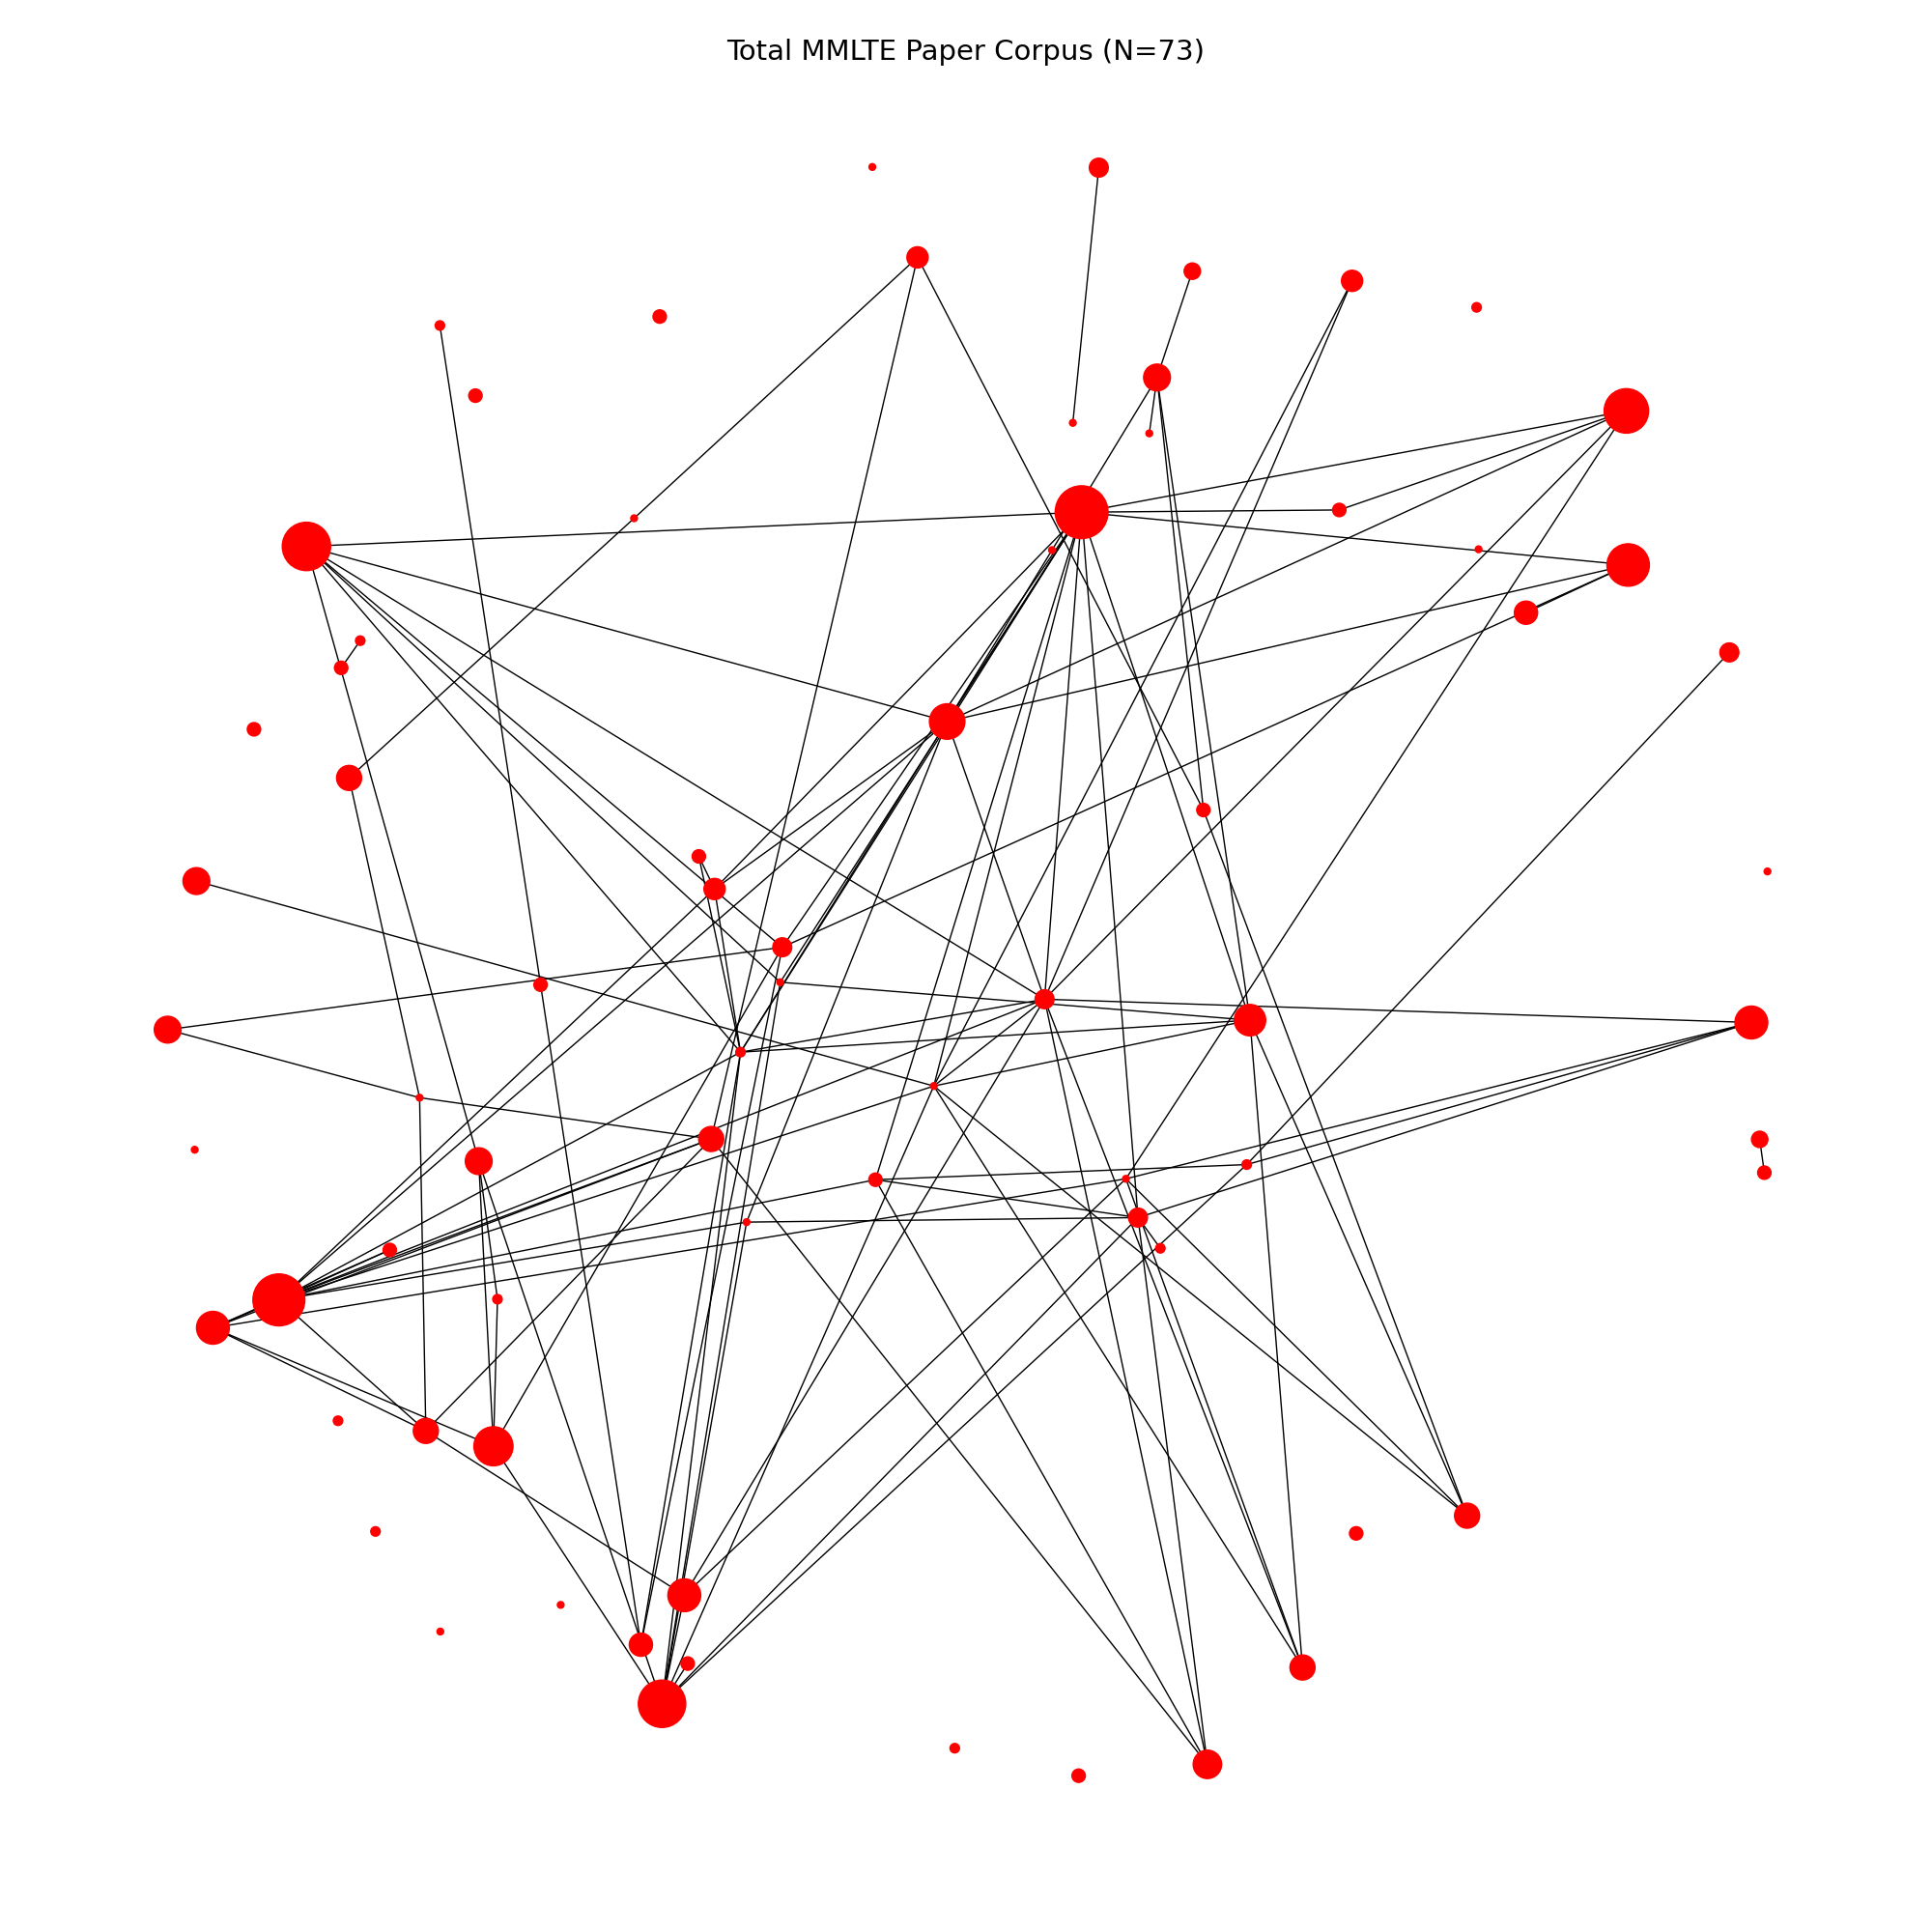
\includegraphics[width=0.5\textwidth, trim=1cm 1cm 1cm 2cm, clip]{img/community_analysis/mmlte_total_corpus_graph.png}
%     \caption{Complete final corpus citation graph: }
%     \label{fig:final_corpus_citation_graph}
% \end{figure}

% For our network approach, we started by using the citation information within our final paper corpus to create a citation graph, shown in Fig. \ref{fig:final_corpus_citation_graph}. Each node is a paper with their weight being their total citation count, rather then their citations within the corpus. This was done to verify that landmark papers were staples both within and outside our corpus.  

% % Identifying Community via Louvain Algorithm
% %   Louvain community discovery algorithm to generate citation communities
% %   Characterized each community via their papers' extracted features
% %   Computed normalized frequency for each category across the communities

% \begin{figure}
%     \centering
%     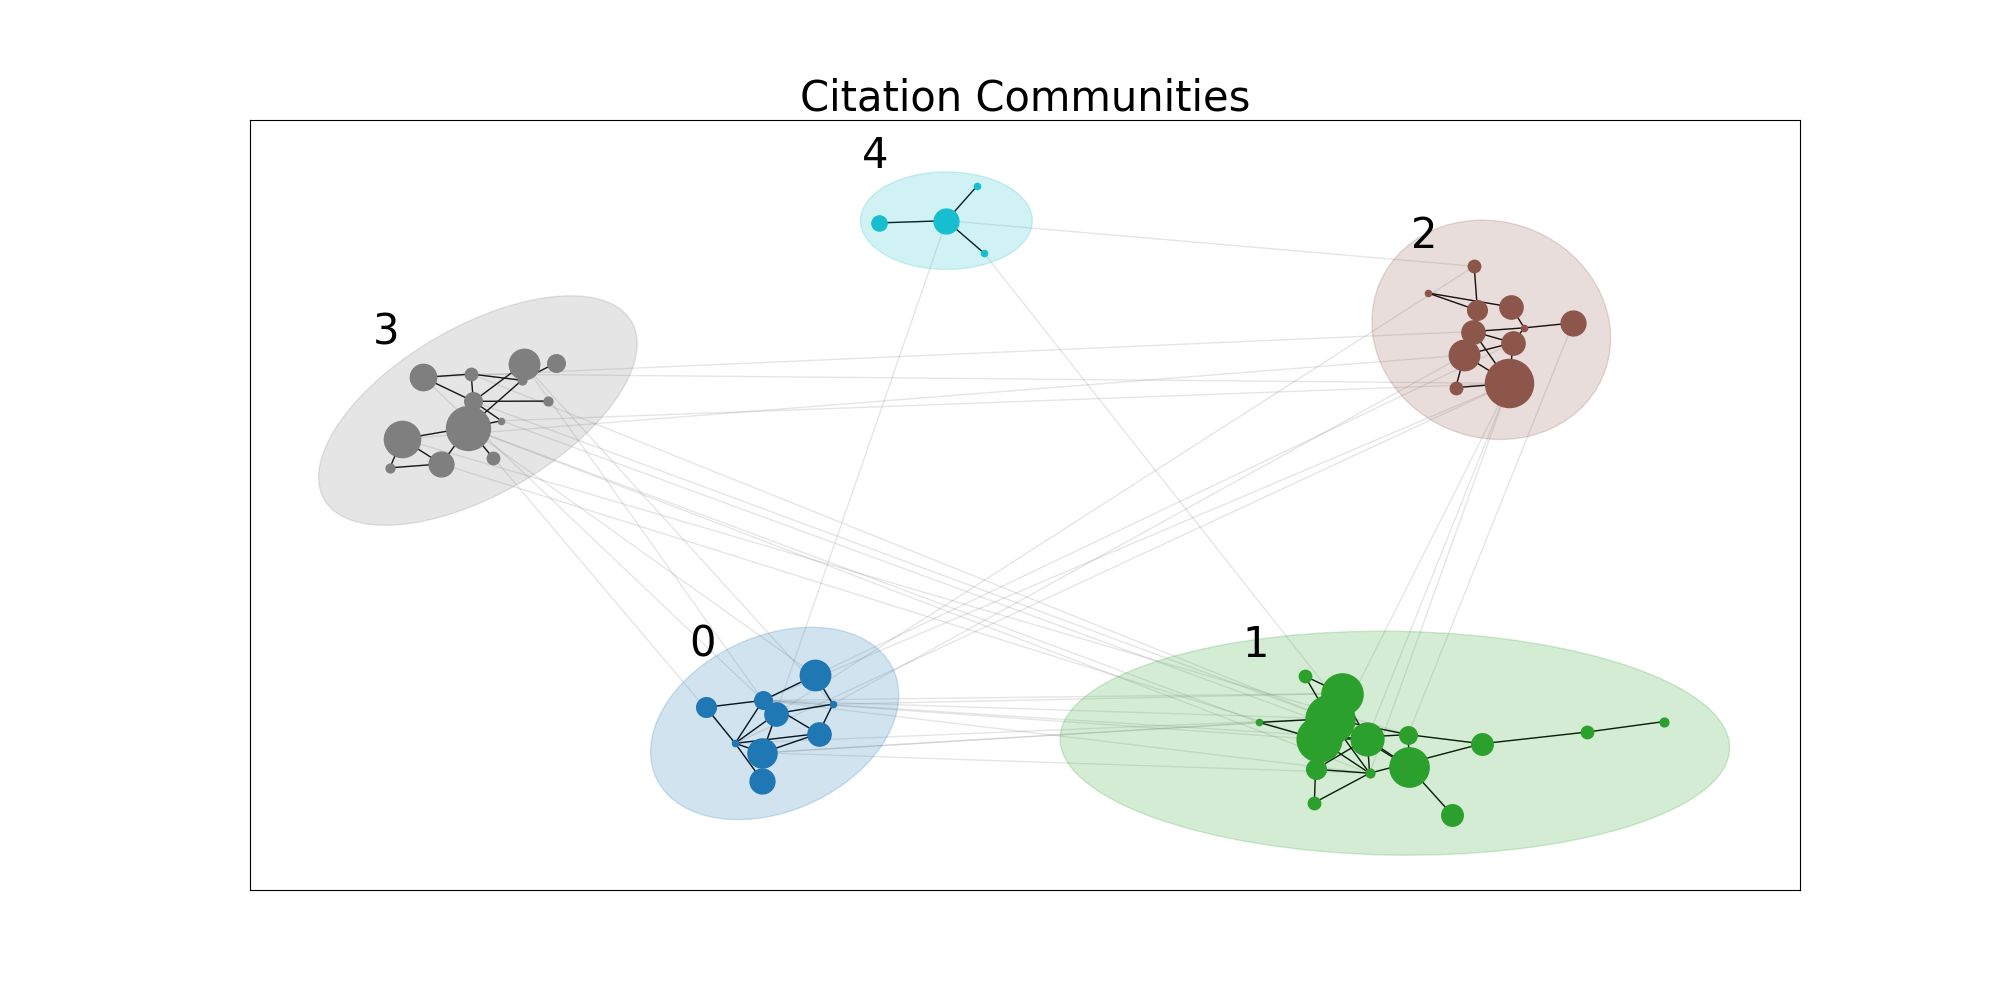
\includegraphics[width=\textwidth, trim=3cm 2cm 3cm 2cm, clip]{img/community_analysis/community_network.png}
%     \caption{Identified citation communities: }
%     \label{fig:citation_communities}
% \end{figure}

% Once with the corpus citation graph constructed, a pre-processing step was performed before using the Louvain algorithm -- Zero degree nodes within the corpus were eliminated to avoid inflating the number of identified communities. By applying the Louvain community algorithm, we obtained eight candidate communities; however, three were discarded for being two-node communities, resulting in five prominent communities. These communities are shown in Fig. \ref{fig:citation_communities}. Understanding how these communities was approached using the discrete circumscribing features through a frequency-based strategy. Across each feature category (e.g. fusion, analysis, modalities), the normalized frequency for each discrete label was computed across each community. To achieve this, each paper's discrete tags were binarized using \href{https://scikit-learn.org/stable/index.html}{Scikit-Learn's} MultiLabelBinarizer. Frequency counts of binary labels were then computed and normalized across community and category. Employing these normalized frequencies, we applied a qualitative approach supported by cosine similarity to hierarchical split communities in an inverted tree fashion, as shown in Fig. \ref{fig:qualitative_breakdown}. Beginning with all communities grouped together, a cosine similarity metric was used to split a group into subgroups by computing the similarity between intra- and inter-groups elements. The splitting processed persisted until a group contained a single community. These groups were then characterized by qualitative observing the normalized frequency differences during each split.

% \begin{figure}
%     \centering
%     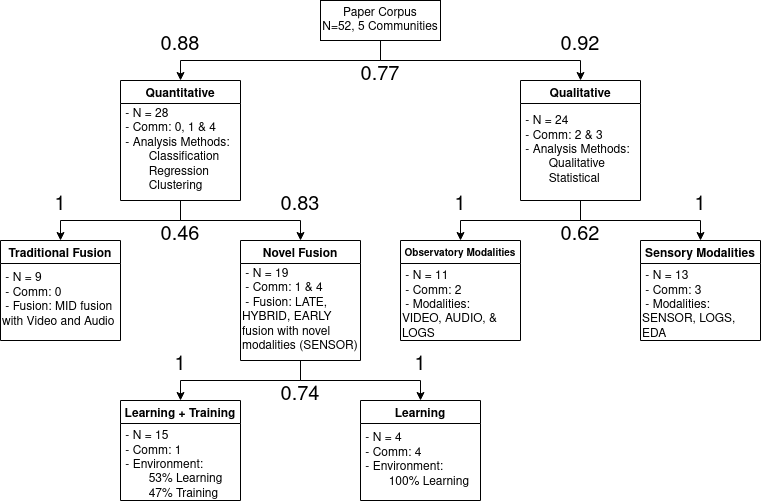
\includegraphics[width=0.8\textwidth]{img/community_analysis/Community Breakdown-Latest.drawio(1).png}
%     \caption{Qualitative breakdown of citation communities using features: }
%     \label{fig:qualitative_breakdown}
% \end{figure}

% \begin{figure}
%     \begin{tabular}{|c|c|}
%         \hline
%         Comm. ID & Papers \\
%         \hline
%         0 & A \\
%         1 & B \\
%         2 & B \\
%         3 & B \\
%         4 & B \\
%         None & \\
%         \hline
%     \end{tabular}
%     \caption{Main caption for the figure}
%     \label{fig:corpus_table}
% \end{figure}

% Beginning of Analysis section describing the communities

% After collecting the final set of papers, we employed various analytical methods to uncover trends, statistics, and clusters in applied MMLA. We started by examining basic descriptive statistics of paper characteristics. Using the citation information from the collected papers, we constructed a citation graph, which served as a basis for further graph-based analysis. We identified graph communities using the Louvain community-finding algorithm from the open-source \href{https://github.com/taynaud/python-louvain}{python-louvain} package. These communities were then described using the circumscribing features, helping us understand specific research subgroups within the field of MMLA.    

% Analysis sections. Will get folded into new framework.

% \subsubsection{Descriptive Statistics}
% % Qualitative analysis via descriptive statistics:
% %   Learning versus training
% %   Fusion types
% %   Analysis types
% %   Modalities
% %       Modalities distribution
% %       # Modalities per paper
% %   Mediums
% %   Publications
% %       Most prevalent publication journals/conferences
% %       Most prevalent publications in our corpus as intersection of union of most cited in corpus and most cited overall

% \section{Findings} \label{sec:findings} 
% % Primary uses of multimodal analysis in MMLTE
% % Discuss the need for mid-fusion versus early fusion

% \subsection{Corpus Statistics}

% % Learning v. training envs
% % Fusion type/bar chart
% % Analysis type/bar chart
% % Modalities bar charts
% % Number of papers per number of modalities
% % Mediums bar charts
% % Publications bar chart

% Limitations piece about original MMLA reference:
% % The term \textit{multimodal learning analytics} was formerly coined in 2013 \cite{blikstein2013multimodal}, and it has experienced increasingly widespread usage in recent years. 

% NLP subdomain raw notes before writing:

% \subsubsection{Natural Language}
% % Descriptive statistics
% % List # of papers falling into this subdomain
% -35 papers use some form of natural language\\

% % List Modalities
% % PROS, TRANS, TEXT, SPECT, AFFECT
% -PROS: 24\\
% -TRANS: 16\\
% -TEXT: 1\\
% -SPECT: 1\\
% -AFFECT: 2

% Vast majority used prosodic audio and transcribed speech. Only 1 for raw text and 1 for audio spectogram.

% Only 8 papers combine PROS and TRANS, and 24 use only one or the other. 

% Most analysis is done via qualitative analysis and statistical methods. Some is done via classification, but not much with reg/patt/net. Contrast to full corpus, where classification was the most prevalent.
% %NLP: {'REG': 6, 'CLS': 14, 'STATS': 21, 'CLUST': 3, 'QUAL': 19, 'PATT': 4, 'NET': 4}

% % ALL: {'CLUST': 9,'QUAL': 29,'CLS': 39,'REG': 12,'STATS': 34,'PATT': 9,'NET': 4}

% Only 9 papers in the entire corpus \textit{only} perform qualitative analysis. 7 of those papers use natural language in some form.
% % Qual only: 
% % NLP: 7/35
% % ALL: 9/73

% Fusion defined in 21/35 papers (60\%) with MID being the favorite. This is less prevalent than the fusion breakdown in the corpus, where ~75\% of papers define fusion (54/73). 
% % NLP: {'MID': 12, 'EARLY': 1, 'OTH': 15, 'HYBRID': 5, 'LATE': 3}
% % OTH fusion only fusion type in 14/35 papers

% % ALL: {'HYBRID': 19, 'LATE': 8, 'MID': 27, 'EARLY': 3, 'OTH': 20}
% % Full corpus OTH fusion only fusion type in 19/73 papers

% No trend among environment settings really except virtual environments less frequent than blended/physical relative to full corpus. Suggests focus on collab in at least some physical space and not 1-on-1 agent interaction, for exanple.
% % NLP: {'PHYS': 13, 'VIRT': 13, 'BLND': 8, 'UNSP': 1}
% % ALL: {'BLND': 20, 'PHYS': 21, 'VIRT': 31, 'UNSP': 2}

% Even with 4:3 ratio of ind to multi in corpus overall, ratio of ind to multi drops to 3:5 with NLP only due to focus on multiperson environments, including conversation. Not surprising given discourse component, but would also be interested in agent-based conversations (which were lacking). 
% % NLP: {'MULTI': 23, 'IND': 14}
% % ALL: {'IND': 45, 'MULTI': 31}

% No trend among didactic nature. relative to overall corpus.
% % NLP: {'INSTR': 21, 'TRAIN': 8, 'INF': 6}
% % ALL: {'INSTR': 45, 'INF': 12, 'UNSP': 1, 'TRAIN': 15}

% Both university and K12, although slight edge to K12 relative to corpus as a whole.
% % NLP: {'UNI': 14, 'K12': 17, 'PROF': 3, 'UNSP': 4}
% % ALL: {'K12': 30, 'UNI': 36, 'UNSP': 7, 'PROF': 5}

% NLP has higher level of model free relative to corpus (17/41, 41\% relative to 27/57, 32\%)
% % NLP: {'MB': 24, 'MF': 17}
% % ALL: {'MB': 57, 'MF': 27}

% Env subjs:
% NLP: {'STEM': 27, 'HUM': 8, 'OTH': 2}
% All: {'STEM': 55, 'HUM': 11, 'UNSP': 4, 'PSY': 5, 'OTH': 2}

% % Results
% %   Example
% -key feature ID relative to outcome (i.e., learning/training gains, skills, confidence, behaviors, strategies, collaboration quality, etc.) (e.g., pauses, n-grams, volume, pitch variation, etc.)
%     -multimodal > unimodal


% % SOTA
% %   Example
% -ML models are the most common quantitative approach: SVM, RF, Logistic regression, linear regression, NB, etc.
%     -Usually used to regress/classify outcome (i.e., performance gains for learning/training)
%     -Other methods used, but sparingly: clustering, behavior patterns, social network analysis, markov chains, etc.
%     -AI methods lacking. DNN methods such as, RNN, LSTM, BERT...but rarer
%     -Traditional NLP methods TF-IDF/Word2Vec used as baselines but not as part of the actual method

% -Qualitative mostly involved descriptive statistics, case studies/individual observations, thematic analysis/constant comparative method of field notes/surveys, qualitative coding

% -Stats: mostly correlation between features and specific features/feature combinations to outcome, and significance testing

% -Lots of collaboration work, evaluating it both on its own and relative to outcome

% % Challenges
% %   Example
% -Hardware/software/multimodal and NLP method limitations for complex tasks (such as characterizing persuasive speech and understanding natural, oral arguments in debate)
%     -Noisy, chaotic environments
%     -ASR mentioned several times
%         -Esp. with adolescents and in noisy environments (cite LID, LAK)
%         -English only
%         -"state-of-the-art diarization system does not perform well on real child-speech interactions"
%     -Speaker diarization
% -Data
%     -Small datasets 
%     -Jargon with domains/children (cite thesis)
% -Complexity
%     -Feature space: "From the audio data, 6405 features were extracted"
% -Opaqueness
% -Time   
%     -Extensive preprocessing and feature engineering required
%     -"a researcher may need to watch screen video data, listen to the audio dialogue several times, and enter behavioural codes into a separate document. Having to do this for every problem and concept students experience over the course of even one class period of learning technology use would be vastly taxing on human time and effort."
%     -"we decided to split the audio manually, which was time consuming and, therefore, led to a lower number of students considered in the applied example."
% -Temporality
%     -Difficult to inform as it unfolds over time
%     -segmentation
%         -"difficulties segmenting the audio files in order to obtain the students-only utterances"

% % Research gaps
% -Lack of textual input. Discuss
% -Only 8 papers use both transcribed audio and prosodic information, which means there is a lack of combining the two
%     -Textless NLP lack with combined audio semantics/prosodic audio
% -Focus on statistical analysis, qualitative, older ML, but lacking in SOTA AI (esp. RL, Transformers, although BERT/Audeering mentioned)
% -Lack of conversational agent-based work. The stuff that's in there doesn't deal with actual conversations between students and agents, as the agent often acts as an evaluator and provides performance metrics or canned responses (i.e., 1-way recommendations) that are not robust to fluid environments  --- and does not act as a mentor, peer, or collaborator.